\documentclass[12pt,a4paper,draft]{article}
\usepackage{tikz}
\usepackage[utf8]{inputenc}
\usepackage{amsmath}
\usepackage{amsfonts}
\usepackage{amssymb}
\usepackage{color}
\definecolor{pblue}{rgb}{0.13,0.13,1}
\definecolor{pgreen}{rgb}{0,0.5,0}
\definecolor{pred}{rgb}{0.9,0,0}
\definecolor{pgrey}{rgb}{0.46,0.45,0.48}
\usepackage[final]{listings}
\lstset{frame=tb,
  language=Java,
  aboveskip=3mm,
  belowskip=3mm,
  showstringspaces=false,
  columns=flexible,
  basicstyle={\small\ttfamily},
  numbers=none,
  breaklines=true,
  breakatwhitespace=true,
  tabsize=3,
  commentstyle=\color{pgreen},
  keywordstyle=\color{pblue},
  stringstyle=\color{pred}
}
\author{Vishal Kedia}
\usepackage{geometry}
\geometry{margin=2cm}
\title{Binary Search Trees}
\begin{document}
\maketitle
\section{Introduction}
The search tree data structures supports many dynamic set operations as mentioned in the API. Hence search trees can be used both as \emph{Dictionaries} and \emph{Priority Queues}
\\
\\
\textbf{Binary Search Tree Property :} Let $x$ be node in a binary search tree. If $y$ is a node in the left sub-tree of $x$, then $y.key \leq x.key$. If $y$ is the node on the right sub-tree of $x$, then $y.key \leq x.key$.
\\
\\
\begin{lstlisting}[caption={Binary Search Tree API}]
public class BST<Key extends Comparable<Key>, Value> {
	private Node root;

	private class Node {
		private Key key;
		private Value value;
		private Node left, right;
		private int N;

		public Node(Key key, Value value, int N) {
			this.key = key;
			this.value = value;
			this.N = N;
		}
	}
	//public void put(Key key, Value value) - Insert operation
	//public Value get(Key key) - Search operation
	//public Key min() - Find the smallest key
	//public Key max() - Find the biggest key
	//public Key predecessor(Key key) - Find the predecessor of the given node
	//public Key successor(Key key) - Find the successor of the given node
	//public void deleteMin() - Delete the smallest key
	//public void deleteMax() - Delete the biggest key
	//public void delete(Key k) - Delete the given key
	//public int size() - Gets the total no of nodes in the given tree
}
\end{lstlisting}
\pagebreak
\section{Operations in BST}
\subsection{Insert in BST}
When inserting a new \texttt{(key,value)} pair in \emph{Binary Search Tree} rooted at $x$, There can be three possible scenarios possible, one where tree is empty, second where tree is not empty but already contains the key and the third scenario where tree is not empty and doesn't contain the any node with the given key.
\par
If the tree is empty then in that case new node with the given key value is returned as root element of the tree. If the Tree is not empty and there is already one node present in the tree with the given key then in that case value of the node in the tree is replaced with new value provided, and if tree is neither empty not contains any node with the provided key then in that case new node is created linked to one of the leaf nodes of in the given tree such that binary search tree property is not violated.

\begin{lstlisting}[caption={Insert Operation}]
private Node root;

public void put(Key key, Value value){
	root = put(root,key,value);
}

private Node put(Node x,Key key,Value value){
	if(Objects.isNull(x)){
		return new Node(key,value,1);
	}else{
		int cmp = key.compareTo(x.key);
		if(cmp < 0){
			x.left = put(x.left,key,value);
		}else if(cmp > 0){
			x.right = put(x.right,key,value);
		}else{
			x.value = value;
		}
		x.N = size(x.left) + size(x.right) + 1;
		return x;
	}
}
\end{lstlisting}
\pagebreak
\subsection{Search in BST}
When we search any key in the given \emph{Binary Search Tree}, then there can be only three possibilities, fist the tree is empty, second when the tree is empty but key doesn't exist and third where tree is not empty and key is present in the tree.

\begin{lstlisting}[caption={Search Operation}]
private Node root;

public Value get(Key key){
	Node node = get(root,key);
	if(Objects.nonNull(node)){
		return node.value;
	}
	return null;
}

private Node get(Node x,Key k){
	if(Objects.isNull(x)){
		return null;
	}
	int cmp = k.compareTo(x.key);
	if(cmp < 0){
		return get(x.left,k);
	}else if(cmp > 0){
		return get(x.right,k);
	}else{
		return x;
	}
}
\end{lstlisting}
\pagebreak
\subsection{Minimum \& Maximum in BST}
The left most element which doesn't have any left child of its own is the minimum and the right most element which doesn't have right child of its own is the maximum in the given \emph{Binary Search Tree}, as per the \emph{Binary Search Tree Property}

\begin{lstlisting}[caption={Min \& Max Operation}]
private Node root;

public Key min(){
	if(Objects.isNull(root)){
		return null;
	}
	return min(root).key;
}

private Node min(Node x){
	if(Objects.isNull(x)){
		return null;
	}
	if(Objects.isNull(x.left)){
		return x;
	}else{
		return min(x.left);
	}
}

public Key max(){
	if(Objects.isNull(root)){
		return null;
	}
	return max(root).key;
}

private Node max(Node x){
	if(Objects.isNull(x)){
		return null;
	}
	if(Objects.isNull(x.right)){
		return x;
	}else{
		return max(x.right);
	}
}
\end{lstlisting}
\pagebreak
\subsection{Predecessor \& Successor in BST}
Predecessor of any given node is the max element in its left sub tree and similarly successor of any given node is the min element in its right sub tree.

\begin{lstlisting}[caption={Predecessor \& Successor Operation}]
private Node root;

public Key predecessor(Key key){
	Node node = get(root,key);
	if(Objects.nonNull(node)){
		Node predecessor = predecessor(node);
		if(Objects.nonNull(predecessor)){
			return predecessor.key;
		}
	}
	return null;
}

private Node predecessor(Node x){
	if(Objects.isNull(x)){
		return null;
	}
	return max(x.left);
}

public Key successor(Key key){
	Node node = get(root,key);
	if(Objects.nonNull(node)){
		Node successor = successor(node);
		if(Objects.nonNull(successor)){
			return successor.key;
		}
	}
	return null;
}

private Node successor(Node x){
	if(Objects.isNull(x)){
		return null;
	}
	return min(x.right);
}	
\end{lstlisting}
\pagebreak
\subsection{Deleting Min \& Max elements in BST}
The left most element is the minimum and the right most element is the maximum in the given \emph{Binary Search Tree}, as per the \emph{Binary Search Tree Property}

\begin{lstlisting}[caption={Deleting Min \& Max Operation}]
private Node root;

public void deleteMin(){
	root = deleteMin(root);
}

private Node deleteMin(Node x){
	if(Objects.isNull(x)){
		return null;
	}
	if(Objects.isNull(x.left)){
		return x.right;
	}
	x.left = deleteMin(x.left);
	return x;
}

public void deleteMax(){
	root = deleteMax(root);
}

private Node deleteMax(Node x){
	if(Objects.isNull(x)){
		return null;
	}
	if(Objects.isNull(x.right)){
		return x.left;
	}
	x.right = deleteMax(x.right);
	return x;
}
\end{lstlisting}
\pagebreak
\subsection{Deleting an element in BST}
Deleting an element from a \emph{Binary Search Tree} is a tricky operation, where in we have to maintain the \emph{Binary Search Tree Property} after deletion by certain adjustments. When we are deleting any given element say $x$ in the BST, Then in that case before deletion we have to find the successor of the element $x$, and assign it a temporary variable say $h$ then point the $x$ left sub tree as $h$  left sub tree. Then delete the successor $h$ from the $x$ right sub tree by calling \textbf{deleteMin} operation on the $x$ right sub tree. And then return the successor element.

\begin{lstlisting}[caption={Delete Operation}]
private Node root;

public void delete(Key k){
	if(k!=null){
		root = delete(root,k);
	}
}

private Node delete(Node x,Key k){
	if(Objects.isNull(x)){
		return x;
	}
	int cmp = k.compareTo(x.key);
	if(cmp < 0){
		return delete(x.left,k);
	}else if(cmp > 0){
		return delete(x.right,k);
	}
	Node succ = successor(x);
	succ.left = x.left;
	succ.right = deleteMin(x.right);
	succ.N = size(succ.left) + size(succ.right);
	return succ;
}
\end{lstlisting}
\section{Binary Search Tree problems}
\subsection{Lowest Common Ancestor Problem (LCA)}
\textbf{Problem Statement -} When we go from node $x$ towards the root element we visit all the ancestors of element $x$, similarly if we visit all the ancestors for the another given element $y$, there will be some intersecting node say $p$ which will be ancestor for both $x$ and $y$ at minimum distance from both $x$ and $y$ making it the \emph{Lowest Common Ancestor} of both the elements. This is also the way to find the minimum distance between the two nodes in a given \emph{Binary Search Tree}.
\\
\textbf{Discussion -} We know from the \emph{Binary Search Tree Property} that all the elements in the left sub tree are smaller than the root element and similarly all the elements in the right sub tree are bigger than the root elements. So if the element $x$ lies in the one sub tree of $p$ and the element $y$ lies on the other sub tree of $p$ then in that case the $p$ is the \emph{LCA} for the elements $x$ and $y$. If we start from the root element then we know if both elements are on the right sub tree then we have to proceed down in the right sub tree to find the \emph{LCA} and if the both the elements are on the left sub tree then we have to proceed down the left sub tree.
\subsection{Algorithm to Test BST}
\textbf{Problem Statement -} You are given a binary tree, device an algorithm to test if the given tree is BST or not.
\\
\textbf{Discussion -} We know that in-order traversal of a BST results in a sorted list of the elements, Hence in order to test we will traverse the tree using in-order traversal and see if all the visited elements are in sorted order or not.
\subsection{BST to DLL (In-Order)}
\textbf{Problem Statement -} Device an algorithm to convert a given BST in a double linked list with In-Order sequence of the elements.
\\
\textbf{Discussion -} To device the above algorithm we have to device two subroutines one to link all the predecessors recursively in the left sub tree and another to link all the successors in the right sub tree recursively.
\par
To link predecessor in the left sub tree delete the max element in the left sub tree and assign an interim pointer to it, now assign the given left sub tree as its left child and then proceed recursively on its left sub tree till you reach empty sub tree, don't forget to store the first predecessor element in the in a global pointer otherwise we will have to traverse till the end to reach the last element as we will have to manipulate its pointers to link with the root element finally. In the similar manner we can link all the successor elements in the right sub tree.
\subsection{BST to DLL (BFS Order)}
\textbf{Problem Statement -} Device an algorithm to convert a given BST in a double linked list with Breadth First Search Order of the elements.
\\
\textbf{Discussion -} For this problem we traverse all the elements in BFS manner using queue, and adjust the pointers while processing all the elements in the queue to form a \emph{Doubly Linked List}.
\subsection{Sorted DLL to BST}
\textbf{Problem Statement-} Device an algorithm to convert a sorted doubly linked list to Binary Search Tree.
\\
\textbf{Discussion -} Since the Doubly Linked List is already sorted, hence if we follow the binary search traversal, over the sorted list and insert the elements as we visit the elements, we can form the balanced BST. The key to the solution is to find the middle element in the least time complexity.
\section{Binary Tree Questions}
\subsection{Creating Binary Tree from given In-Order and Pre-Order Sequence of the elements}
\textbf{Problem Statement -}Device an algorithm to re-create a binary tree from the given In-Order and Pre-Order sequence of the elements of the tree.
\\
\textbf{Discussion -}As we know that the in Pre-Order sequence the first element is the root element in the tree, using this information we can divide the In-Order sequence in three parts, first the root element itself, second the left subtree elements and third the right subtree elements. And using the above result we know all the elements present in the left sub tree and the right sub tree and we can derive the pre order sequence of those elements from the given Pre-Order sequence and solve the problem recursively.
\subsection{Diameter of a Binary Tree}
\textbf{Problem Statement -}Diameter of a given binary tree is given as the number of nodes on the longest path between the two leave nodes which may or may not pass through the root element. There can be multiple paths with the same node numbers.
\\
\textbf{Discussion -}As we know that the height of a binary tree is the longest path between the root node and the leaf node, so in case of the diameter if the longest path between the two nodes passes throught the given node then in that case diameter is the sum of the height of the left and the right sub trees plus $1$. Since we don't know if the longest path passes through the root element of the given tree hence we have to test for all the elements as the root elements for diameter and then choose the one with the longest diameter.
\subsection{Full Nodes in Binary Tree}
\textbf{Problem Statement -} Full Node in a binary tree is the node which has non null left and the right sub trees. Device an algorithm to count the no of full nodes in a binary tree.
\subsection{Half Nodes in Binary Tree}
\textbf{Problem Statement -} Half Node in a binary tree is the node which has only one child sub tree. Device an algorithm to count the no of all the half nodes in a binary tree.
\subsection{Height of a Binary Tree}
\textbf{Problem Statement -} Height of a binary tree is defined as the number of nodes in the longest path between the root of the tree and any of the leaf nodes. Device an algorithm to determine the height of the binary tree.
\subsection{Print All Ancestors}
\textbf{Problem Statement -} Device an algorithm to print all the ancestors of the given node in a binary tree.
\subsection{Print All Leaf Node Paths}
\textbf{Problem Statement -} Device an algorithm to print all the leaf node paths in the given binary tree.
\subsection{Size of the Binary Tree}
\textbf{Problem Statement -} Size of a binary tree is defined as the total no of nodes present in the tree. Device an algorithm to find the size of a given binary tree.
\subsection{Test for structural identity}
\textbf{Problem Statement -} Device an algorithm to test if the two given binary trees are structurally identical or not.
\subsection{Tree Mirror}
\textbf{Problem Statement -} Device an algorithm to create mirror image of the given binary tree.
\begin{tikzpicture}
\draw (0,0) circle [radius=10pt] node(a){1};
\draw (-1,-1) circle [radius=10pt] node(b){3};
\draw (1,-1) circle [radius=10pt] node(c){2};
\draw (0,-2) circle [radius=10pt] node(f){5};
\draw (2,-2) circle [radius=10pt] node(g){4};
\draw (a) -- (b);
\draw (a) -- (c);
\draw (c) -- (f);
\draw (c) -- (g);
\draw [thick,dash dot](5,1) -- (5,-5);
\draw (10,0) circle [radius=10pt] node(A){1};
\draw (9,-1) circle [radius=10pt] node(B){2};
\draw (11,-1) circle [radius=10pt] node(C){3};
\draw (8,-2) circle [radius=10pt] node(D){4};
\draw (10,-2) circle [radius=10pt] node(E){5};
\draw (A) -- (B);
\draw (A) -- (C);
\draw (B) -- (D);
\draw (B) -- (E);
\end{tikzpicture}
\subsection{Sum of vertical nodes in Binary Trees}
\textbf{Problem Statement -}  Device an algorithm to calculate the sum of all the vertical nodes in the given binary tree. In the below example if we see, then nodes are $1$,$5$,$6$ are vertically aligned.
\\
\begin{center}
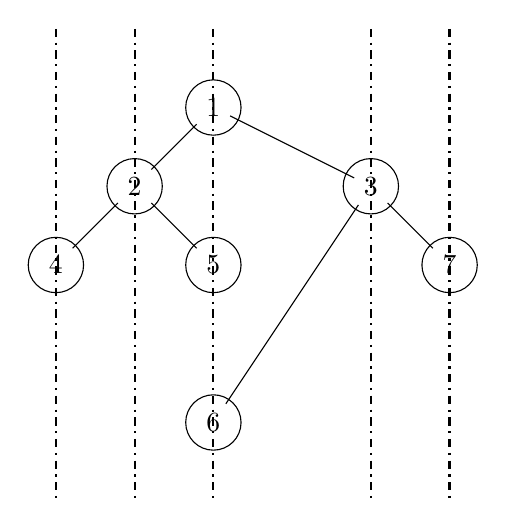
\begin{tikzpicture}
\draw [thick,dash dot](-2,1) -- (-2,-5);
\draw [thick,dash dot](-1,1) -- (-1,-5);
\draw [thick,dash dot](0,1) -- (0,-5);
\draw [thick,dash dot](2,1) -- (2,-5);
\draw [thick,dash dot](3,1) -- (3,-5);
\draw (0,0) circle [radius=10pt] node(a){1};
\draw (-1,-1) circle [radius=10pt] node(b){2};
\draw (2,-1) circle [radius=10pt] node(c){3};
\draw (0,-4) circle [radius=10pt] node(f){6};
\draw (3,-2) circle [radius=10pt] node(g){7};
\draw (-2,-2) circle [radius=10pt] node(d){4};
\draw (0,-2) circle [radius=10pt] node(e){5};
\draw (a) -- (b);
\draw (a) -- (c);
\draw (b) -- (d);
\draw (b) -- (e);
\draw (c) -- (f);
\draw (c) -- (g);
\end{tikzpicture}
\end{center}
\pagebreak
\subsection{Level Order Tree Traversal in Spiral Form (ZigZag Traversal)}
\textbf{Problem Statement -} Traverse the below tree in level order spiral form such that it visits in the order 1,2,3,7,6,5,4.
\begin{center}
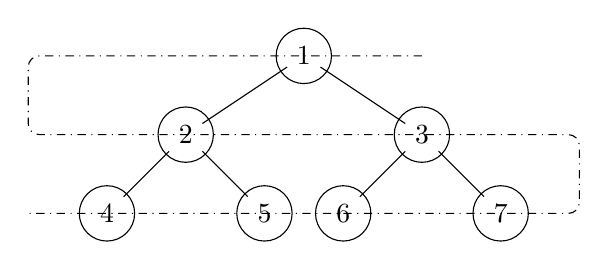
\begin{tikzpicture}
\draw (-.5,0) circle [radius=10pt] node(a){1};
\draw (-2,-1) circle [radius=10pt] node(b){2};
\draw (1,-1) circle [radius=10pt] node(c){3};
\draw (0,-2) circle [radius=10pt] node(f){6};
\draw (2,-2) circle [radius=10pt] node(g){7};
\draw (-3,-2) circle [radius=10pt] node(d){4};
\draw (-1,-2) circle [radius=10pt] node(e){5};
\draw (a) -- (b);
\draw (a) -- (c);
\draw (b) -- (d);
\draw (b) -- (e);
\draw (c) -- (f);
\draw (c) -- (g);
\draw [rounded corners,dash dot](1,0) -- (-4,0) -- (-4,-1) -- (3,-1) -- (3,-2) -- (-4,-2);
\end{tikzpicture}
\end{center}
\subsection{Closes Leaf in a Binary Tree}
\textbf{Problem Statement -} You are given a binary tree and a key, find the closest leaf from that tree in the given binary tree, eg. In the below tree $B$ is the closest leaf to key $C$ and the distance is $2$.
\begin{center}
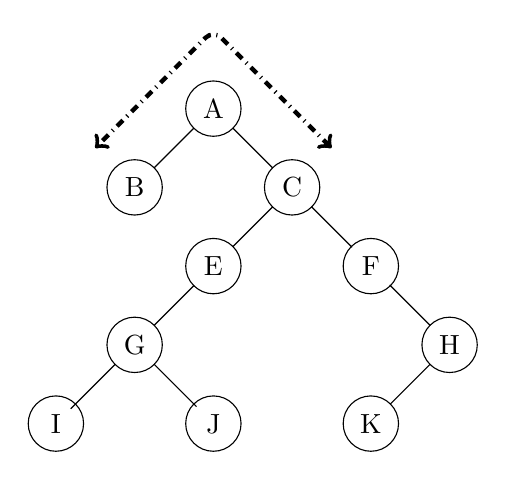
\begin{tikzpicture}
\draw (0,0) circle [radius=10pt] node(a){A};
\draw (-1,-1) circle [radius=10pt] node(b){B};
\draw (a) -- (b);
\draw (1,-1) circle [radius=10pt] node(c){C};
\draw (a) -- (c);
\draw (0,-2) circle [radius=10pt] node(e){E};
\draw (c) -- (e);
\draw (-1,-3) circle [radius=10pt] node(g){G};
\draw (e) -- (g);
\draw (-2,-4) circle [radius=10pt] node(i){I};
\draw (g) -- (i);
\draw (0,-4) circle [radius=10pt] node(j){J};
\draw (g) -- (j);
\draw (2,-2) circle [radius=10pt] node(f){F};
\draw (c) -- (f);
\draw (3,-3) circle [radius=10pt] node(h){H};
\draw (f) -- (h);
\draw (2,-4) circle [radius=10pt] node(k){K};
\draw (h) -- (k);
\draw[rounded corners,dash dot,ultra thick,<->] (1.5,-0.5) -- (0,1) -- (-1.5,-0.5);
\end{tikzpicture}
\end{center}
\textbf{Discussion -}If we think a little, its easier to observe that closest leaf to the key is either in its descendant or path to the closest key passes via one of its ancestors. So, we will have to search the given key in the binary tree, and keep the track of all the ancestors along with the direction how we reached the key. Once we reach the given key, we shall find the nearest leaf in the sub tree rooted at the given tree and store the distance in a variable say $p$; now we to revisit at least $k-1$ ancestors one by one, and seek the closest leaf in the left sub tree of the ancestor if the search key was in the right sub tree or if the search key was in the left sub tree of the ancestor then we have to find the closest leaf in the right sub tree of the ancestor and store the result in $x$ then the distance of the closest leaf from the search key becomes $y=2+x$ and we keep the $p=min(y,p)$ we will repeat this until $k-1$ ancestors are visited if the number of ancestors are more than $k-1$ or till all the ancestors are visited and in the end return the value of $p$.
\pagebreak
\subsection{Equal Tree Partition}
\textbf{Problem Statement -}If given a binary tree with $n$ nodes, check if by removing any link in the tree we may partition the tree into two trees such that the sum of all the nodes in both the trees are equal.
\begin{center}
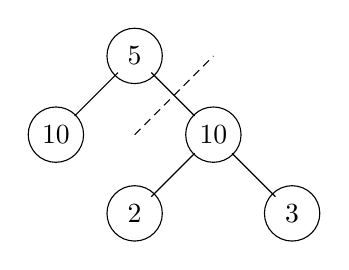
\begin{tikzpicture}
\draw (0,0) circle [radius=10pt] node(a){5};
\draw (-1,-1) circle [radius=10pt] node(b){10};
\draw (1,-1) circle [radius=10pt] node(c){10};
\draw (0,-2) circle [radius=10pt] node(d){2};
\draw (2,-2) circle [radius=10pt] node(e){3};
\draw (a) -- (b);
\draw (a) -- (c);
\draw (c) -- (d);
\draw (c) -- (e);
\draw[densely dashed] (0,-1) -- (1,0);
\end{tikzpicture}
\end{center}
\textbf{Discussion -} In this problem we will have to find the sum of all the elements in the tree considering each element in the given binary tree as the root element forming a tree of its own, and store that value in the extra variable in each node for the corresponding tree. Now if we observe, we find that whenever any link is cut in the given tree the parent tree gets broken in two tree, one with the original root element of the main tree and another with the broken link element which doesn't have any ancestor. Since we have stored the sum of all the elements for the given tree in the root node, so once the tree is broken to get the remaining value we have to subtract it with the total sum stored in the root element in the another sub tree that will give the sum of all the elements in the remaining sub tree. We have to perform this operation for all the elements in the given tree and see which two partitions leads to the same sum, and that shall be our required partition.
\subsection{Longest Consecutive Sequence in Binary Tree}
\textbf{Problem Statement -}Given a Binary Tree, find the length of the longest path which comprises of nodes with consecutive values in increasing order. Every node is to be considered a path of length $1$.
\subsection{Boundry Traversal of a Binary Tree}
\textbf{Problem Statement -}  
\end{document}
